
	Se presenta el esquema del filtro propuesto en la Figura \ref{fig:filtro_adaptativo}. 
	Ambos sistemas (el desconocido y el filtro adaptativo) se excitan con una señal de referencia $u(n)$ de ruido blanco gaussiano.
	Luego se computa la diferencia entre ambas salidas y se utiliza esta señal de error para el ajuste de los parámetros del filtro mediante algún algoritmo adaptativo.
	Cuando el filtro aprenda a comportarse igual que el sistema a identificar, el error será bajo, y los coeficientes del filtro podrán utilizarse como estimadores de los parámetros del sistema a identificar.

\vspace*{\fill}
\begin{figure}[H]
\centering
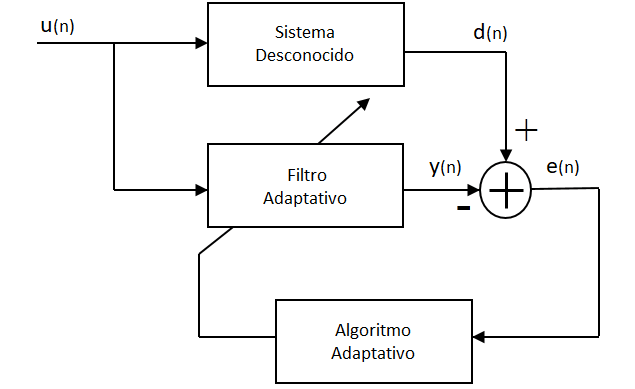
\includegraphics[scale=0.5]{filtro_adaptativo.png}
\caption{Filtro Adatptativo.}
\label{fig:filtro_adaptativo} 
\end{figure}
\vspace*{\fill}

Ahora bien, esto tiene un problema. La salida del filtro adaptativo se computa de la siguiente manera:
\begin{equation*}
	y(n) = w^T U(n)
\end{equation*}
donde $U(n) = [u(n) \> u(n - 1) \> ... \> u(n - M + 1)]^T$, $M$ es el orden del filtro y $w$ son los coeficientes del mismo.

	Ésto significa que el filtro adaptativo propuesto sólo sirve para estimar la respuesta en frecuencia de sistemas FIR y el sistema bajo análisis tiene la forma de un filtro IIR en tiempo discreto:

\begin{equation*}
		x_{0}(n) = b_{0} \> x_{1}(n) + b_{1} \> x_{1}(n - 1) + a_{0} \> x_{0}(n - 1) + a_{1} \> x_{0}(n - 2)
\end{equation*}

Una posible solución a esto es, en lugar de sólo introducir ruido blanco a la entrada, combinar el ruido blanco con algunos valores pasados de la salida:

\begin{equation*}
	U(n) = [x_{1}(n) \> x_{1}(n - 1) \> x_{0}(n - 1) \> x_{0}(n - 2)]^T
\end{equation*}

Donde ahora se excita al sistema con $x_{1}$ ruido blanco gaussiano. Ahora los coeficientes $w$ ajustados del filtro podrán utilizarse como estimadores:

\begin{equation*}
	[w_{0} \> w_{1} \> w_{2} \> w_{3}]^T  = [\hat{b}_{0} \> \hat{b}_{1} \> \hat{a}_{0} \> \hat{a}_{1}]^T
\end{equation*}

Ahora bien, como estos coeficientes son función de las constantes $M$, $b$ y $k$, pueden estimarse las mismas. El unico componente que falta es la elección del algoritmo adaptativo. Se propone en principio utilizar el algoritmo LMS, que obtiene los parametros $w$ de la siguiente manera:

\begin{equation*}
	w(n) = w(n - 1) + \mu \> U(n) \> [d(n) - U(n)^* w(n - 1)]
\end{equation*}

donde $\mu$ es una constante de aprendizaje.
